\documentclass{standalone}
\usepackage{tikz}
\usetikzlibrary{patterns, positioning}

\begin{document}
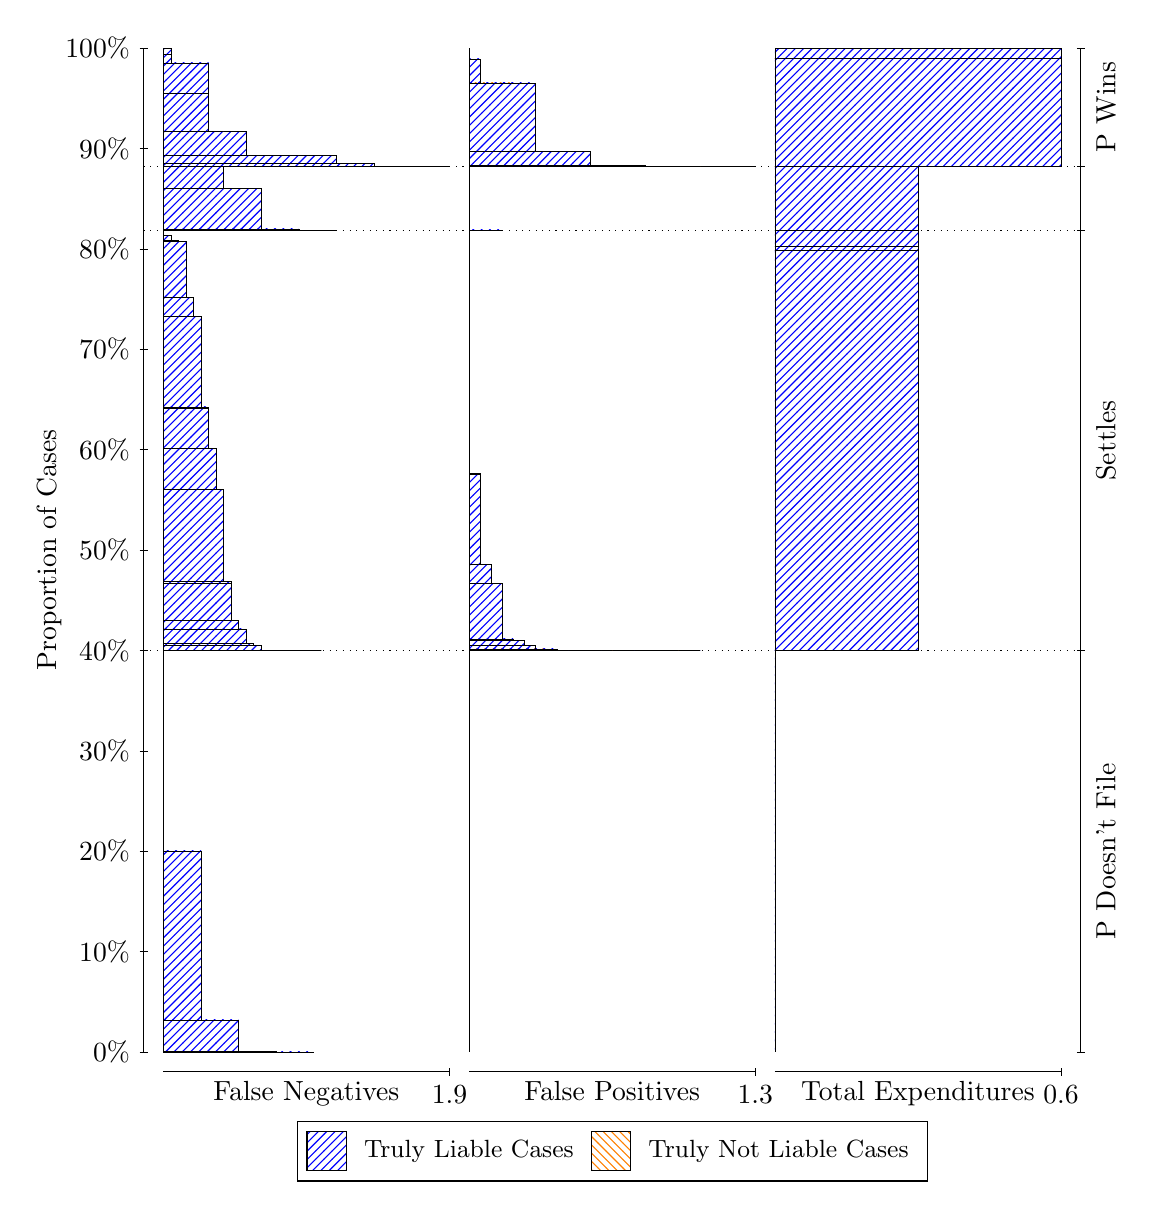
\begin{tikzpicture}
\draw[black, very thin] (1.5,1.75) -- (1.5,14.5);
\node[rotate=90, anchor=center] at (0.3, 8.125) {Proportion of Cases};
\draw[black, very thin] (1.45,1.75) -- (1.55,1.75);
\node[anchor=east] at (1.45, 1.75) {0\%};
\draw[black, very thin] (1.45,3.025) -- (1.55,3.025);
\node[anchor=east] at (1.45, 3.025) {10\%};
\draw[black, very thin] (1.45,4.3) -- (1.55,4.3);
\node[anchor=east] at (1.45, 4.3) {20\%};
\draw[black, very thin] (1.45,5.575) -- (1.55,5.575);
\node[anchor=east] at (1.45, 5.575) {30\%};
\draw[black, very thin] (1.45,6.85) -- (1.55,6.85);
\node[anchor=east] at (1.45, 6.85) {40\%};
\draw[black, very thin] (1.45,8.125) -- (1.55,8.125);
\node[anchor=east] at (1.45, 8.125) {50\%};
\draw[black, very thin] (1.45,9.4) -- (1.55,9.4);
\node[anchor=east] at (1.45, 9.4) {60\%};
\draw[black, very thin] (1.45,10.675) -- (1.55,10.675);
\node[anchor=east] at (1.45, 10.675) {70\%};
\draw[black, very thin] (1.45,11.95) -- (1.55,11.95);
\node[anchor=east] at (1.45, 11.95) {80\%};
\draw[black, very thin] (1.45,13.225) -- (1.55,13.225);
\node[anchor=east] at (1.45, 13.225) {90\%};
\draw[black, very thin] (1.45,14.5) -- (1.55,14.5);
\node[anchor=east] at (1.45, 14.5) {100\%};

\draw[black, very thin] (13.4,1.75) -- (13.4,14.5);
\draw[black, very thin] (13.35,1.75) -- (13.45,1.75);
\node[anchor=west] at (13.35, 1.75) {};
\draw[black, very thin] (13.35,6.8489) -- (13.45,6.8489);
\node[anchor=west] at (13.35, 6.8489) {};
\draw[black, very thin] (13.35,12.187) -- (13.45,12.187);
\node[anchor=west] at (13.35, 12.187) {};
\draw[black, very thin] (13.35,12.999) -- (13.45,12.999);
\node[anchor=west] at (13.35, 12.999) {};
\draw[black, very thin] (13.35,14.5) -- (13.45,14.5);
\node[anchor=west] at (13.35, 14.5) {};

\draw[black, very thin, pattern color=blue, pattern=north east lines] (1.75,1.75) rectangle (3.6623,1.75);
\draw[black, very thin, pattern color=blue, pattern=north east lines] (1.75,1.75) rectangle (3.1842,1.7534);
\draw[black, very thin, pattern color=blue, pattern=north east lines] (1.75,1.7534) rectangle (2.7061,2.158);
\draw[black, very thin, pattern color=blue, pattern=north east lines] (1.75,2.158) rectangle (2.2281,4.3029);
\draw[black, very thin, pattern color=orange, pattern=north west lines] (1.75,4.3029) rectangle (1.75,4.3029);
\draw[black, very thin, pattern color=blue, pattern=north east lines] (1.75,4.3029) rectangle (1.75,6.8489);
\draw[black, very thin, pattern color=blue, pattern=north east lines] (1.75,6.8489) rectangle (3.7579,6.8489);
\draw[black, very thin, pattern color=blue, pattern=north east lines] (1.75,6.8489) rectangle (3.5667,6.8489);
\draw[black, very thin, pattern color=blue, pattern=north east lines] (1.75,6.8489) rectangle (3.3754,6.8489);
\draw[black, very thin, pattern color=blue, pattern=north east lines] (1.75,6.8489) rectangle (3.2798,6.8498);
\draw[black, very thin, pattern color=blue, pattern=north east lines] (1.75,6.8498) rectangle (3.1842,6.8502);
\draw[black, very thin, pattern color=blue, pattern=north east lines] (1.75,6.8502) rectangle (3.0886,6.8509);
\draw[black, very thin, pattern color=blue, pattern=north east lines] (1.75,6.8509) rectangle (2.993,6.9158);
\draw[black, very thin, pattern color=blue, pattern=north east lines] (1.75,6.9158) rectangle (2.8974,6.9357);
\draw[black, very thin, pattern color=blue, pattern=north east lines] (1.75,6.9357) rectangle (2.8018,7.1245);
\draw[black, very thin, pattern color=blue, pattern=north east lines] (1.75,7.1245) rectangle (2.7061,7.2308);
\draw[black, very thin, pattern color=blue, pattern=north east lines] (1.75,7.2308) rectangle (2.6105,7.7082);
\draw[black, very thin, pattern color=blue, pattern=north east lines] (1.75,7.7082) rectangle (2.6105,7.7218);
\draw[black, very thin, pattern color=blue, pattern=north east lines] (1.75,7.7218) rectangle (2.5149,8.8988);
\draw[black, very thin, pattern color=blue, pattern=north east lines] (1.75,8.8988) rectangle (2.4193,9.4168);
\draw[black, very thin, pattern color=blue, pattern=north east lines] (1.75,9.4168) rectangle (2.3237,9.9189);
\draw[black, very thin, pattern color=blue, pattern=north east lines] (1.75,9.9189) rectangle (2.3237,9.9417);
\draw[black, very thin, pattern color=blue, pattern=north east lines] (1.75,9.9417) rectangle (2.2281,11.096);
\draw[black, very thin, pattern color=blue, pattern=north east lines] (1.75,11.096) rectangle (2.1325,11.335);
\draw[black, very thin, pattern color=blue, pattern=north east lines] (1.75,11.335) rectangle (2.1325,11.335);
\draw[black, very thin, pattern color=blue, pattern=north east lines] (1.75,11.335) rectangle (2.0368,12.04);
\draw[black, very thin, pattern color=blue, pattern=north east lines] (1.75,12.04) rectangle (1.9412,12.047);
\draw[black, very thin, pattern color=blue, pattern=north east lines] (1.75,12.047) rectangle (1.9412,12.061);
\draw[black, very thin, pattern color=blue, pattern=north east lines] (1.75,12.061) rectangle (1.8456,12.121);
\draw[black, very thin, pattern color=blue, pattern=north east lines] (1.75,12.121) rectangle (1.8456,12.121);
\draw[black, very thin, pattern color=blue, pattern=north east lines] (1.75,12.121) rectangle (1.75,12.121);
\draw[black, very thin, pattern color=orange, pattern=north west lines] (1.75,12.121) rectangle (1.75,12.121);
\draw[black, very thin, pattern color=blue, pattern=north east lines] (1.75,12.121) rectangle (1.75,12.187);
\draw[black, very thin, pattern color=blue, pattern=north east lines] (1.75,12.187) rectangle (3.9491,12.187);
\draw[black, very thin, pattern color=blue, pattern=north east lines] (1.75,12.187) rectangle (3.4711,12.204);
\draw[black, very thin, pattern color=blue, pattern=north east lines] (1.75,12.204) rectangle (2.993,12.721);
\draw[black, very thin, pattern color=blue, pattern=north east lines] (1.75,12.721) rectangle (2.5149,12.996);
\draw[black, very thin, pattern color=blue, pattern=north east lines] (1.75,12.996) rectangle (2.0368,12.999);
\draw[black, very thin, pattern color=orange, pattern=north west lines] (1.75,12.999) rectangle (1.75,12.999);
\draw[black, very thin, pattern color=blue, pattern=north east lines] (1.75,12.999) rectangle (5.3833,12.999);
\draw[black, very thin, pattern color=blue, pattern=north east lines] (1.75,12.999) rectangle (4.9053,12.999);
\draw[black, very thin, pattern color=blue, pattern=north east lines] (1.75,12.999) rectangle (4.4272,13.035);
\draw[black, very thin, pattern color=blue, pattern=north east lines] (1.75,13.035) rectangle (3.9491,13.133);
\draw[black, very thin, pattern color=blue, pattern=north east lines] (1.75,13.133) rectangle (3.7579,13.133);
\draw[black, very thin, pattern color=blue, pattern=north east lines] (1.75,13.133) rectangle (3.4711,13.135);
\draw[black, very thin, pattern color=blue, pattern=north east lines] (1.75,13.135) rectangle (3.2798,13.136);
\draw[black, very thin, pattern color=blue, pattern=north east lines] (1.75,13.136) rectangle (2.993,13.136);
\draw[black, very thin, pattern color=blue, pattern=north east lines] (1.75,13.136) rectangle (2.8018,13.442);
\draw[black, very thin, pattern color=blue, pattern=north east lines] (1.75,13.442) rectangle (2.5149,13.442);
\draw[black, very thin, pattern color=blue, pattern=north east lines] (1.75,13.442) rectangle (2.3237,13.921);
\draw[black, very thin, pattern color=blue, pattern=north east lines] (1.75,13.921) rectangle (2.3237,14.311);
\draw[black, very thin, pattern color=blue, pattern=north east lines] (1.75,14.311) rectangle (1.8456,14.415);
\draw[black, very thin, pattern color=blue, pattern=north east lines] (1.75,14.415) rectangle (1.8456,14.492);
\draw[black, very thin, pattern color=orange, pattern=north west lines] (1.75,14.492) rectangle (1.75,14.492);
\draw[black, very thin, pattern color=blue, pattern=north east lines] (1.75,14.492) rectangle (1.75,14.5);
\draw[black, very thin, pattern color=orange, pattern=north west lines] (5.6333,1.75) rectangle (5.6333,1.75);
\draw[black, very thin, pattern color=blue, pattern=north east lines] (5.6333,1.75) rectangle (5.6333,6.8489);
\draw[black, very thin, pattern color=orange, pattern=north west lines] (5.6333,6.8489) rectangle (8.5679,6.8489);
\draw[black, very thin, pattern color=blue, pattern=north east lines] (5.6333,6.8489) rectangle (8.5679,6.8489);
\draw[black, very thin, pattern color=orange, pattern=north west lines] (5.6333,6.8489) rectangle (8.2885,6.8489);
\draw[black, very thin, pattern color=blue, pattern=north east lines] (5.6333,6.8489) rectangle (8.2885,6.8489);
\draw[black, very thin, pattern color=orange, pattern=north west lines] (5.6333,6.8489) rectangle (8.009,6.8489);
\draw[black, very thin, pattern color=blue, pattern=north east lines] (5.6333,6.8489) rectangle (8.009,6.8489);
\draw[black, very thin, pattern color=blue, pattern=north east lines] (5.6333,6.8489) rectangle (7.8692,6.8489);
\draw[black, very thin, pattern color=orange, pattern=north west lines] (5.6333,6.8489) rectangle (7.7295,6.8489);
\draw[black, very thin, pattern color=blue, pattern=north east lines] (5.6333,6.8489) rectangle (7.7295,6.8489);
\draw[black, very thin, pattern color=blue, pattern=north east lines] (5.6333,6.8489) rectangle (7.5897,6.8489);
\draw[black, very thin, pattern color=orange, pattern=north west lines] (5.6333,6.8489) rectangle (7.45,6.8489);
\draw[black, very thin, pattern color=blue, pattern=north east lines] (5.6333,6.8489) rectangle (7.45,6.8489);
\draw[black, very thin, pattern color=blue, pattern=north east lines] (5.6333,6.8489) rectangle (7.3103,6.8489);
\draw[black, very thin, pattern color=orange, pattern=north west lines] (5.6333,6.8489) rectangle (7.1705,6.8489);
\draw[black, very thin, pattern color=blue, pattern=north east lines] (5.6333,6.8489) rectangle (7.1705,6.8489);
\draw[black, very thin, pattern color=orange, pattern=north west lines] (5.6333,6.8489) rectangle (7.1705,6.8489);
\draw[black, very thin, pattern color=blue, pattern=north east lines] (5.6333,6.8489) rectangle (7.1705,6.8489);
\draw[black, very thin, pattern color=blue, pattern=north east lines] (5.6333,6.8489) rectangle (7.0308,6.8489);
\draw[black, very thin, pattern color=blue, pattern=north east lines] (5.6333,6.8489) rectangle (6.891,6.8489);
\draw[black, very thin, pattern color=orange, pattern=north west lines] (5.6333,6.8489) rectangle (6.891,6.8489);
\draw[black, very thin, pattern color=blue, pattern=north east lines] (5.6333,6.8489) rectangle (6.891,6.8489);
\draw[black, very thin, pattern color=blue, pattern=north east lines] (5.6333,6.8489) rectangle (6.7513,6.8688);
\draw[black, very thin, pattern color=orange, pattern=north west lines] (5.6333,6.8688) rectangle (6.6115,6.8688);
\draw[black, very thin, pattern color=blue, pattern=north east lines] (5.6333,6.8688) rectangle (6.6115,6.87);
\draw[black, very thin, pattern color=blue, pattern=north east lines] (5.6333,6.87) rectangle (6.4718,6.9151);
\draw[black, very thin, pattern color=blue, pattern=north east lines] (5.6333,6.9151) rectangle (6.4718,6.9151);
\draw[black, very thin, pattern color=orange, pattern=north west lines] (5.6333,6.9151) rectangle (6.3321,6.9151);
\draw[black, very thin, pattern color=blue, pattern=north east lines] (5.6333,6.9151) rectangle (6.3321,6.9749);
\draw[black, very thin, pattern color=blue, pattern=north east lines] (5.6333,6.9749) rectangle (6.1923,6.9888);
\draw[black, very thin, pattern color=blue, pattern=north east lines] (5.6333,6.9888) rectangle (6.1923,6.996);
\draw[black, very thin, pattern color=blue, pattern=north east lines] (5.6333,6.996) rectangle (6.0526,7.7006);
\draw[black, very thin, pattern color=blue, pattern=north east lines] (5.6333,7.7006) rectangle (5.9128,7.9404);
\draw[black, very thin, pattern color=blue, pattern=north east lines] (5.6333,7.9404) rectangle (5.7731,9.089);
\draw[black, very thin, pattern color=blue, pattern=north east lines] (5.6333,9.089) rectangle (5.7731,9.0942);
\draw[black, very thin, pattern color=blue, pattern=north east lines] (5.6333,9.0942) rectangle (5.6333,12.187);
\draw[black, very thin, pattern color=orange, pattern=north west lines] (5.6333,12.187) rectangle (6.0526,12.187);
\draw[black, very thin, pattern color=blue, pattern=north east lines] (5.6333,12.187) rectangle (6.0526,12.19);
\draw[black, very thin, pattern color=blue, pattern=north east lines] (5.6333,12.19) rectangle (5.6333,12.999);
\draw[black, very thin, pattern color=orange, pattern=north west lines] (5.6333,12.999) rectangle (9.2667,12.999);
\draw[black, very thin, pattern color=blue, pattern=north east lines] (5.6333,12.999) rectangle (9.2667,12.999);
\draw[black, very thin, pattern color=orange, pattern=north west lines] (5.6333,12.999) rectangle (8.5679,12.999);
\draw[black, very thin, pattern color=blue, pattern=north east lines] (5.6333,12.999) rectangle (8.5679,12.999);
\draw[black, very thin, pattern color=orange, pattern=north west lines] (5.6333,12.999) rectangle (7.8692,12.999);
\draw[black, very thin, pattern color=blue, pattern=north east lines] (5.6333,12.999) rectangle (7.8692,13.006);
\draw[black, very thin, pattern color=orange, pattern=north west lines] (5.6333,13.006) rectangle (7.1705,13.006);
\draw[black, very thin, pattern color=blue, pattern=north east lines] (5.6333,13.006) rectangle (7.1705,13.188);
\draw[black, very thin, pattern color=blue, pattern=north east lines] (5.6333,13.188) rectangle (6.4718,14.056);
\draw[black, very thin, pattern color=orange, pattern=north west lines] (5.6333,14.056) rectangle (6.1923,14.056);
\draw[black, very thin, pattern color=blue, pattern=north east lines] (5.6333,14.056) rectangle (6.1923,14.056);
\draw[black, very thin, pattern color=blue, pattern=north east lines] (5.6333,14.056) rectangle (5.7731,14.362);
\draw[black, very thin, pattern color=orange, pattern=north west lines] (5.6333,14.362) rectangle (5.6333,14.362);
\draw[black, very thin, pattern color=blue, pattern=north east lines] (5.6333,14.362) rectangle (5.6333,14.5);
\draw[black, very thin, pattern color=orange, pattern=north west lines] (9.5167,1.75) rectangle (9.5167,1.75);
\draw[black, very thin, pattern color=blue, pattern=north east lines] (9.5167,1.75) rectangle (9.5167,6.8489);
\draw[black, very thin, pattern color=orange, pattern=north west lines] (9.5167,6.8489) rectangle (11.333,6.8489);
\draw[black, very thin, pattern color=blue, pattern=north east lines] (9.5167,6.8489) rectangle (11.333,11.926);
\draw[black, very thin, pattern color=orange, pattern=north west lines] (9.5167,11.926) rectangle (11.333,11.926);
\draw[black, very thin, pattern color=blue, pattern=north east lines] (9.5167,11.926) rectangle (11.333,11.985);
\draw[black, very thin, pattern color=orange, pattern=north west lines] (9.5167,11.985) rectangle (11.333,11.985);
\draw[black, very thin, pattern color=blue, pattern=north east lines] (9.5167,11.985) rectangle (11.333,12.187);
\draw[black, very thin, pattern color=orange, pattern=north west lines] (9.5167,12.187) rectangle (11.333,12.187);
\draw[black, very thin, pattern color=blue, pattern=north east lines] (9.5167,12.187) rectangle (11.333,12.999);
\draw[black, very thin, pattern color=orange, pattern=north west lines] (9.5167,12.999) rectangle (13.15,12.999);
\draw[black, very thin, pattern color=blue, pattern=north east lines] (9.5167,12.999) rectangle (13.15,14.364);
\draw[black, very thin, pattern color=orange, pattern=north west lines] (9.5167,14.364) rectangle (13.15,14.364);
\draw[black, very thin, pattern color=blue, pattern=north east lines] (9.5167,14.364) rectangle (13.15,14.5);
\draw[black, dotted] (1.5,6.8489) -- (13.4,6.8489);
\draw[black, dotted] (1.5,12.187) -- (13.4,12.187);
\draw[black, dotted] (1.5,12.999) -- (13.4,12.999);
\draw[black, very thin] (1.75,1.5) -- (5.3833,1.5);
\node[anchor=north] at (3.5667, 1.5) {False Negatives};
\draw[black, very thin] (5.3833,1.45) -- (5.3833,1.55);
\node[anchor=north] at (5.3833, 1.45) {1.9};

\draw[black, very thin] (5.6333,1.5) -- (9.2667,1.5);
\node[anchor=north] at (7.45, 1.5) {False Positives};
\draw[black, very thin] (9.2667,1.45) -- (9.2667,1.55);
\node[anchor=north] at (9.2667, 1.45) {1.3};

\draw[black, very thin] (9.5167,1.5) -- (13.15,1.5);
\node[anchor=north] at (11.333, 1.5) {Total Expenditures};
\draw[black, very thin] (13.15,1.45) -- (13.15,1.55);
\node[anchor=north] at (13.15, 1.45) {0.6};

\node[black, centered, rotate=90] at (13.72, 4.2994) {P Doesn't File};
\node[black, centered, rotate=90] at (13.72, 9.518) {Settles};

\node[black, centered, rotate=90] at (13.72, 13.749) {P Wins};

\draw (7.449999999999999,1.5) node[draw=none] (baseCoordinate) {};
\begin{scope}[align=center]
        \matrix[scale=0.5, draw=black, below=0.5cm of baseCoordinate, nodes={draw}, column sep=0.1cm]{
            \node[rectangle, draw, minimum width=0.5cm, minimum height=0.5cm, pattern=north east lines, pattern color=blue] {}; &
            \node[draw=none, font=\small] (B) {Truly Liable Cases}; &
            \node[rectangle, draw, minimum width=0.5cm, minimum height=0.5cm, pattern=north west lines, pattern color=orange] {}; &
            \node[draw=none, font=\small] (B) {Truly Not Liable Cases}; \\
            };
\end{scope}

\end{tikzpicture}
\end{document}